\documentclass[11pt]{article}

\usepackage{mathtools}
\usepackage{amssymb}
\usepackage{amsmath}
\usepackage{amsthm}
\usepackage{hyperref}
\usepackage{microtype}
\usepackage{graphicx}
\graphicspath{ {./img/} }

\setlength{\parindent}{0cm}
\let\emptyset\varnothing

\title{\textbf{CSCI/MATH 2113 Discrete Structures} \\ Chapter 5 Relations and Functions}
\author{Alyssa Motas}

\begin{document}

    \maketitle

    \pagebreak

    \tableofcontents

    \pagebreak

    \section{(5.1) Cartesian Products and Relations}

        \subsection{Cartesian Product}

        \subsubsection{Definition}
        For sets $A, B$ the \emph{Cartesian product}, or \emph{cross product}, of $A$ and $B$ is denoted by \(A \times B\) and equals \(\{(a,b) \mid a \in A, b \in B\}.\)

        \subsubsection{Example}
        Suppose that \(A = \{2,3,4\}\) and \(B = \{4,5\}\) then we have \[A \times B = \{(2,4),(2,5),(3,4),(3,5),(4,4),(4,5)\}.\] Note that \[A \times B \neq B \times A.\] Another example of a Cartesian product is the real plane \(\mathbb{R} \times \mathbb{R}\).

        \subsubsection{Notation}
        \[A^n = \underbrace{A \times A \times A \times \dots \times A}_\text{$n$ times}.\]

        \subsection{Relations}

        \subsubsection{Definition}
        For sets $A, B$, any subset of \(A \times B\) is called a (\emph{binary}) \emph{relation} from $A$ to $B$. Any subset of \(A \times A\) is called a (\emph{binary}) \emph{relation} on $A$.

        \subsubsection{Notation}
        If $R$ is a relation on $A$ and \((a,a') \in R\), then we write \(a R a'\). 

        \subsubsection{Examples}
        Suppose that \(A = \{2,3,4\}\) and \(B = \{4,5\}\). Then,
        \begin{itemize}
            \item \(\{(2,5),(2,4)\}\)
            \item \(A \times B\)
            \item \(\emptyset\)
        \end{itemize}
        are relations from $A$ to $B$.

        \subsubsection{Counting}
        For finite sets $A,B$ with \(|A| = m\) and \(|B| = n\), there are \(2^{mn}\) relations from $A$ to $B$, including the empty relation as well as the relation \(A \times B\) itself.

        \vspace{1em}

        There are also \(2^{nm} (= 2^{mn})\) relations from $B$ to $A$, one of which is also \(\emptyset\) and another of which is \(B \times A\). The reason we get the same number of relations from $B$ to $A$ as we have from $A$ to $B$ is that any relation \(R_1\) from $B$ to $A$ can be obtained from a unique relation $R_2$ from $A$ to $B$ by simply reversing the components of each ordered pair in $R_2$ (and vice versa).

        \subsubsection{Standard Relations}
        Standard relations can be expressed in this way: \[R = \{(a,b) \in \mathbb{Z} \times \mathbb{Z} \mid b = a + n \text{ for } n \in \mathbb{N}\}.\] This is the relation ``is less than or equal to.'' Indeed \[(a,b) \in R \text{ if and only if } a \leq b.\] Suppose that \(A = \{1\}\) and let \(R \subseteq \mathcal{P}(A)^2\) defined by \[R = \{(\emptyset, \emptyset), (\emptyset, \{1\}), (\{1\}, \{1\})\}.\] This is the relation ``is a subset of.'' Indeed, \[(S,S') \in R \text{ if and only if } S \subseteq S'.\]

        \subsubsection{Theorem}
        For sets $A$, $B$, and $C$:
        \begin{itemize}
            \item \(A \times \emptyset = \emptyset = \emptyset \times A\)
            \item \(A \times (B \cap C) = (A \times B) \cap (A \times C)\)
            \item \(A \times (B \cup C) = (A \times B) \cup (A \times C)\)
            \item \((B \cap C) \times A = (B \times A) \cap (C \times A)\)
            \item \((B \cup C) \times A = (B \times A) \cup (C \times A)\)
        \end{itemize}
        \begin{proof}
            Let \(x \in A \times (B \cap C)\). Then \(x = (a,d)\) when \(a \in A, d \in B \cap C\). So, \(x = (a,d)\) with \(a \in A\) and \(d \in B\) which implies that \(x \in A \times B.\) But \(x = (a,d)\) with \(a \in A\) and \(d \in C\), which implies \(x \in A \times C\). Hence, we have \(x \in (A \times B) \cap (A \times C)\) which implies \(A \times (B \cap C) \subseteq (A \times B) \cap (A \times C).\) The converse inclusion is shown similarly. Hence we have the desired equality. The other statements are proved similarly as well.
        \end{proof}

        \subsubsection{Recursive Relation}
        An example of a recursively defined relation is on \(\mathbb{N} \times \mathbb{N}\):
        \begin{enumerate}
            \item \((0,0) \in R\)
            \item If \((s,t) \in R\) then \((s+1, t+7) \in R\).
        \end{enumerate}
        In fact, we have \[R = \{(m,n) \mid n = 7m\}.\]

        
    \section{(5.2) Functions Plain and One-to-One}

        \subsection{Defintion of a function}

        For nonempty sets $A$, $B$, a \emph{function}, or \emph{mapping}, $f$ from $A$ to $B$, denoted \(f: A \rightarrow B\), is a relation from $A$ to $B$ in which every lement of $A$ appears exactly once as the first component of an ordered pair in the relation. 

        \vspace{1em}

        We have \(f \subseteq A \times B\) and 
        \begin{enumerate}
            \item[(1)] Existence: \[\forall a \in A, \exists b \in B, (a,b) \in f.\]
            \item[(2)] Uniqueness: If \((a,b) \in f\) and \((a,b') \in f\) then \[b = b'.\]   
        \end{enumerate}

        \subsubsection{Image and Preimage}

        If \((a,b) \in f\), we write \(f(a)=b\). We then say that $b$ is the \emph{image} of $a$ under $f$, and that $a$ is the \emph{preimage} of $b$ under $f$.

        \vspace{1em}

        \emph{Example.} The absolute value is the function \(|x|: \mathbb{R} \rightarrow \mathbb{R}\). Here, 2 and -2 are two preimages of 2 since \[|2| = 2 = |-2|.\] So a given element can have more than one preimage.

        \subsubsection{Domain and codomain}

        For the function \(f: A \rightarrow B\), $A$ is called the \emph{domain} of $f$ and $B$ the \emph{codomain} of $f$. The subset of $B$ consisting of those elements that appear as second components in the ordered pairs of $f$ is called the \emph{range} of $f$ and is also denoted by $f(A)$ because it is the set of images (of the elements of $A$) under $f$.

        \vspace{1em}

        \emph{Note:} Range does not imply that it is equal to codomain.

        \subsubsection{Examples}

        \begin{enumerate}
            \item The \emph{greatest integer function}, or \emph{floor function}. This function \(f: \mathbb{R \rightarrow \mathbb{R}}\), is given by \[f(x) = \lfloor x \rfloor = \text{ the greatest integer less than or equal to $x$}\] \emph{Example.} \(\lfloor 7.7 + 8.4 \rfloor = \lfloor 16.1 \rfloor = 16.\)
            \item The \emph{ceiling function}. This function \(g: \mathbb{R} \rightarrow \mathbb{Z}\) is defined by \[g(x) = \lceil x \rceil = \text{ the least integer greater than or equal to $x$.}\] \emph{Example.} \(\lceil 3.3 + 4.2 \rceil = \lceil 7.5 \rceil = 8.\)
            \item The function trunc (for truncation). It deletes the fractional part of a real number. Note that trunc(3.78) = \(\lfloor 3.78 \rfloor = 3\) while trunc(-3.78) = \(\lceil -3.78 \rceil = -3.\)
            \item The \emph{access} function. In storing a matrix in a one-dimensional array, many computer languages use the \emph{row major} implementation. If \(A = (a_{ij})_{m \times n}\) is an \(m \times n\) matrix, to determine the location of an entry \(a_{ij}\) from $A$, where \(1 \leq i \leq m, 1 \leq j \leq n\), we can use the formula for the access function: \[f(a_{ij}) = (i - 1)n + j.\]
        \end{enumerate}

        \subsubsection{Counting functions}

        Let \(A,B\) be nonempty sets with \(|A| = m, |B| = n.\) How many functions are there in \(f:A \rightarrow B\)?

        \vspace{1em}

        Suppose that \(A = \{a_1, a_2, a_3, \dots, a_m\}\) and \(B = \{b_1, b_2, b_3, \dots, b_n\}\), then a typical function can be described by \(\{(a_1, x_1), (a_2,x_2), \dots, (a_m, x_m)\}.\) We can select any $n$ elements of $B$ for \(x_1\) then do the same for \(x_2\). We continue this selection until one of the $n$ elements of $B$ is finally selected for \(x_m\). Using the product rule, there are \[n^m = |B|^{|A|}\] functions from $A$ to $B$.

        \vspace{1em}

        \emph{Example.} Suppose that \(A = \{1,2,3\}\) and \(B = \{w,x,y,z\}\). There are \(4^3 = 64\) functions from $A$ to $B$.

        \vspace{1em}

        In general, we do not expect \(|A|^{|B|} = |B|^{|A|}\).

        \subsection{One-to-one Correspondence}

        \subsubsection{Definition}

        A function \(f:A \rightarrow B\) is called \emph{one-to-one}, or \emph{injective}, if each element of $B$ appears at most once as the image of an element of $A$. 
        
        \vspace{1em}

        If \(f: A \rightarrow B\) is one-to-one, with $A$, $B$ finite, we must have \(|A| \leq |B|\). For arbitrary sets \(A,B\), \(f: A \rightarrow B\) is one-to-one if and only if for all \(a_1, a_2 \in A, f(a_1) = f(a_2) \Rightarrow a_1 = a_2.\) Consequently, we also have \(a_1 \neq a_2 \Rightarrow f(a_1) \neq f(a_2).\)

        \subsubsection{Examples}

        \begin{enumerate}
            \item Suppose that \(f: \mathbb{R} \rightarrow \mathbb{R}\) where \(f(x) = 3x + 7\) for all \(x \in \mathbb{R}\). Then for all \(x_1,x_2 \in \mathbb{R}\), we find that \[f(x_1) = f(x_2) \Rightarrow 3x_1 + 7 = 3x_2 + 7 \Rightarrow 3x_1 = 3x_2 \Rightarrow x_1 = x_2,\] so the given function $f$ is one-to-one.
            \item Suppose that \(g: \mathbb{R} \rightarrow \mathbb{R}\) is the function defined by \(g(x) = x^4 - x\) for each real number $x$. Then \[g(0) = (0)^4 - 0 = 0 \text{ and } g(1) = (1)^4 - (1) = 1 - 1 = 0.\] Consequently, $g$ is not one-to-one since \(g(0) = g(1)\) but \(0 \neq 1.\)
        \end{enumerate}

        \subsubsection{Counting injective functions}

        Let \(A,B\) be nonempty sets with \(|A| = m, |B| = n.\) How many injective functions are there in \(f:A \rightarrow B\)?

        \vspace{1em}

        Suppose that \(A = \{a_1, \dots, a_m\}\), \(B = \{b_1, \dots, b_n\}\), and that \(m \leq n\). The one-to-one function has the form \(\{(a_1,x_1), \dots, (a_m, x_m)\}\), where there are $n$ choices for \(x_1\), \(n-1\) choices for \(x_2\), \(n-2\) choices for \(x_3\), and so on, finishing with \(n - (m - 1) = n - m + 1\) choices for \(x_m\). By the rule of product, we have \[n(n-1)(n-2) \dots (n - m + 1) = \frac{n!}{(n - m)!} = P(n,m) = P(|B|,|A|).\]

        \subsubsection{Direct Image}

        If \(f: A \rightarrow B\) and \(A_1 \subseteq A\), then \[f(A_1) = f[A_1] = \{b \in B \mid b = f(a), \text{ for some } a \in A_1\},\] and \(f(A_1)\) is called the \emph{direct image} of \(A_1\) under $f$.

        \vspace{1em}

        \emph{Example.} Let \(g: \mathbb{R} \rightarrow \mathbb{R}\) be given by \(x^2\). Then \(g(\mathbb{R}) = \text{ the range of $g$ } = [0, + \infty).\) The \emph{image} of \(\mathbb{Z}\) under $g$ is \[g(\mathbb{Z}) = \{0,1,4,9,16, \dots\}\] and for \(A_1 = [-2,1]\) we get \[g(A_1) = [0,4].\]

        \subsubsection{Set Operations}

        Let \(f: A \rightarrow B\), with \(A_1, a_2 \subseteq A\). Then
        \begin{enumerate}
            \item[(a)] \(f(A_1 \cup A_2) = f(A_1) \cup f(A_2);\)
            \item[(b)] \(f(A_1 \cap A_2) \subseteq f(A_1) \cap f(A_2)\);
            \item[(c)] \(f(A_1 \cap A_2) = f(A_1) \cap f(A_2)\) when $f$ is one-to-one.   
        \end{enumerate}
        \begin{proof}
            Part (b): For each \(b \in B, b \in f(A_1 \cap A_2) \Rightarrow b = f(a),\) for some \(a \in A_1 \cap A_2 \implies [b = f(a) \text{ for some } a \in A_1]\) and \([b = f(a) \text{ for some } a \in A_2] \Rightarrow b \in f(A_1)\) and \(b \in f(A_2) \Rightarrow b \in f(A_1) \cap f(A_2)\), so \(f(A_1 \cap A_2) \subseteq f(A_1) \cap f(A_2)\).
        \end{proof}

        \subsubsection{Restriction}

        If \(f: A \rightarrow B\) and \(A_1 \subseteq A\), then \(f |_{A_1} : A_1 \rightarrow B\) is called the \emph{restriction of f to $A_1$} if \(f|_{A_1}(a) = f(a)\) for all \(a \in A_1\).
        
        \subsubsection{Extension}

        Let \(A_1 \subseteq A\) and \(f:A_1 \rightarrow B.\) If \(g:A \rightarrow B\) and \(g(a) = f(a)\) for all \(a \in A_1\), then we call $g$ an \emph{extension of f to A}.

    \section{(5.3) Onto Functions Stirling Numbers of the Second Kind}

    \subsection{Surjective Functions}
    \subsubsection{Definition}

    \(f: A \rightarrow B\) is \emph{onto} or \emph{surjective} if \(\forall b \in B, \exists a \in A\) such that \(f(a)=b.\)

    \vspace{1em}

    \emph{Remark.} A function is onto if its range is equal to the codomain. 

    \vspace{1em}

    If \(A,B\) are finite sets, then for an onto function \(f: A \rightarrow B\) to possibly exist we must have \(|A| \leq |B|\). 

    \subsubsection{Examples}
    \begin{itemize}
        \item For the function \(f: \mathbb{R} \rightarrow \mathbb{R}\) defined by \(f(x)=x^3\) we have: if \(x \in \mathbb{R}\), then \(f(\sqrt[3]x) = (\sqrt[3]x)^3 = x.\) This means that $f$ is onto.
        \item For the function \(g: \mathbb{R} \rightarrow \mathbb{R}\) defined by \(g(x)=x^2\) we have: no such \(y \in \mathbb{R}\) that satisfies \(y^2 = -1.\) For instance, \[g(x) = x^2 = -9 \Rightarrow r = 3i, -3i \in \mathbb{C}.\] Therefore, $g$ is not onto.
    \end{itemize}

    \subsubsection{Counting}

    Suppose that \(A = \{x,y,z\}\) and \(B = \{1,2\}\). How many \(f: A \rightarrow B\) are onto? 
    \begin{proof}
        The function \(f: A \rightarrow B\) is not onto if and only if \(f(a) = 1\) for all \(a \in A\) or \(f(a)=2\) for all \(a \in A\). Hence, the number we seek is \[|B|^{|A|} - 2 = 2^3 - 2 = 6.\]
    \end{proof}
    In general, if $A$ and $B$ are sets with \(|A| = m\) and \(|B| = n\), then this quantity is \[ \sum_{k = 0}^{n} (-1)^k \binom{n}{n - k} (n-k)^m \] onto functions from $A$ to $B$.

    \subsection{Stirling Numbers}

    \subsubsection{A combinatorial interpretation}

    In how many ways can you distribute 4 objects into 3 labelled cotainers with no container empty?
    We just need to count the number of surjections from $A$ to $B$. By the previuos formula, this is \[\sum_{k = 0}^{3} (-1)^k \binom{3}{3-k} (3-k)^4 = 36.\] What if we had the same situation but with containers that aren't labelled? The number of such distributions is \[S(m,n) = \frac{1}{n!} \sum_{k=0}^n (-1)^k \binom{n}{n-k} (n-k)^m\] where the factor of \(\frac{1}{n!}\) corrects for the fact that certain distributions are equivalent.

    So \(S(m,n)\) is the number of ways to distribute $m$ objects into $n$ identical containers with no container left empty. 

    \subsubsection{Definition}

    \(S(m,n)\) is a \emph{Stirling number} of the 2nd kind.
    
    \section{(5.4) Special Functions}

    \subsection{Binary operations}
    \subsubsection{Definition}

    For any nonempty sets \(A,B\), any function \(f: A \times A \rightarrow B\) is called \emph{binary operation} on $A$. If \(B \subseteq A\), then the binrary operation is said to be \emph{closed} (on $A$). (When \(B \subseteq A\) we may also say that $A$ is \emph{closed under f}.)

    \vspace{1em}

    \emph{Remark.} Similarly, \(f : A^n \rightarrow B\) is an \emph{n-ary} operation on $A$. When $n=1$, the operation is \emph{unary} or \emph{monary}.

    \subsubsection{Examples of Binary Operations}
    \begin{itemize}
        \item For \(f: \mathbb{Z} \times \mathbb{Z} \rightarrow \mathbb{Z}\) defined by \(f(a,b) = a - b\), it is a closed binary operation on \(\mathbb{Z}\).
        \item For \(g: \mathbb{Z} \times \mathbb{Z} \rightarrow \mathbb{R}\) defined by \(g(a,b) = a^b\), it is a non-closed binary operation.
        \item For \(h: \mathbb{Z} \times \mathbb{Z} \rightarrow \mathbb{R}\) defined by \(h(a,b) = a + b\), it is a binary operation.
        \item For \(j: \mathcal{P}(A) \times \mathcal{P}(A) \rightarrow \mathcal{P}(A)\) defined by \(j(S,T) = S \cup T\), it is a closed binary operation.
        \item For \(k: \mathcal{P}(A) \rightarrow \mathcal{P}(A)\) defined by \(k(S) = S^c\), it is a closed unary operation.
    \end{itemize}

    \subsubsection{Commutativity and Associativity}
    Let \(f: A \times A \rightarrow B\); that is, $f$ is a binary operation on $A$.
    \begin{enumerate}
        \item[(a)] $f$ is said to be \emph{commutative} if \(f(a,b) = f(b,a)\) for all \((a,b) \in A \times A.\)
        \item[(b)] When \(B \subseteq A\) (that is, when $f$ is closed), $f$ is said tot be $associative$ if for all \(a,b,c \in A, f(f(a,b),c) = f(a,f(b,c)).\)  
    \end{enumerate}

    \subsubsection{Examples of Commutativity and Associativity}
    
    Binary operations that are both commutative and associative:
    \begin{itemize}
        \item + on \(\mathbb{Z}\): \(n + m = m + n\) and \(n + (m + r) = (n + m) + r\)
        \item \(\times\) on \(\mathbb{Z}\)
        \item \(\cup\) on \(\mathcal{P}(A)\)
    \end{itemize}

    Binary operations that are associative but not commutative:
    \begin{itemize}
        \item \(\times\) on \(Mat_{n \times n}(\mathbb{R})\) which is the multiplication of $n \times n$ real matrices.
    \end{itemize}


    Binary operations that are both not commutative and associative:
    \begin{itemize}
        \item \(-\) on \(\mathbb{Z}\): \[2 - 3 = -1 \neq 1 = 3 - 2\] \[((3-3) - 2) = -2 \neq 2 = 3 - (3 - 2) \]
    \end{itemize}

    \subsubsection{Symmetry}

    Suppose that \(f: A \times A \rightarrow A\) is a binary operation where \(A = \{a_1, \dots, a_n\}\). We can represent $f$ using a \emph{table}.
    \begin{center}
        \begin{tabular}{| c | c | c | c | c |} \hline
            $f$      & $a_1$        & $a_2$        & $\dots$ & $a_n$        \\ \hline
            $a_1$    & $f(a_1,a_1)$ & $f(a_1,a_2)$ &         &              \\ \hline
            $a_2$    & $f(a_2,a_1)$ &              &         &              \\ \hline
            $\vdots$ &              &              &         &              \\ \hline
            $a_n$    &              & $f(a_n,a_2)$ &         & $f(a_n,a_n)$ \\ \hline
            
        \end{tabular}
    \end{center}
    If the operation is commutative, then the table is \emph{symmetric.}

    Now let \(f: \{a,b,c\} \times \{a,b,c\} \rightarrow \{a,b,c\}\) be defined by the table:
    \begin{center}
        \begin{tabular}{| c | c | c | c |} \hline
            $f$ & $a$ & $b$ & $c$ \\ \hline
            $a$ & $b$ & $a$ & $a$ \\ \hline
            $b$ & $a$ & $c$ & $a$ \\ \hline
            $c$ & $a$ & $a$ & $c$ \\ \hline
        \end{tabular}
    \end{center}
    Here we have \[f(a,f(b,c)) = f(a,a) = b \neq a = f(a,c) = f(f(a,b),c)\] so the operation is \emph{not associative} but it is commutative since the table is symmetric.

    \subsection{Identity Element}

    \subsubsection{Definition}

    Let \(f: A \times A \rightarrow B\) be a binary operation on $A$. An element \(x \in A\) is called an \emph{identity} (or \emph{identity element}) for $f$ if \(f(a,x) = f(x,a) = a\), for all \(a \in A\).

    \subsubsection{Examples}

    \begin{itemize}
        \item 0 for + on \(\mathbb{Z}\) since \[a + 0 = 0 + a = a\] for all \(a \in \mathbb{Z}\).
        \item \(I_n\) (identity matrix) of $x$ on \(Mat_{n \times n} (\mathbb{R})\).
        \item \(\emptyset\) for \(\cup\) on \(\mathcal{P}(A)\).
        \item $A$ for \(\cap\) on \(\mathcal{P}(A)\).
    \end{itemize}

    \subsubsection{Theorem}

    Let \(f : A \times A \rightarrow B\) be a binary operation. If $f$ has an identity, then that identity is unique.
    \begin{proof}
        If $f$ has more than one identity, let \(x_1, x_2 \in A\) with
        \begin{align*}
            f(a, x_1) = a = f(x_1,a), && \text{for all } a \in A, \\
            f(a, x_2) = a = f(x_2,a), && \text{for all } a \in A.
        \end{align*}
        Consider \(x_1\) as an element of $A$ and $x_2$ as an identity. Then \(f(x_1,x_2) = x_1\). Now reverse the roles of \(x_1\) and \(x_2\), that is, consider \(x_2\) as an element of $A$ and $x_1$ as an identity. We find that \(f(x_1,x_2) = x_2\). Consequently, \(x_1 = x_2\), and $f$ has at most one identity.
    \end{proof}

    \subsection{Projections}

    For sets $A$ and $B$, if \(D \subseteq A \times B\), then \(\pi_A : D \rightarrow A\), defined by \(\pi_A (a,b) = a\), is called the \emph{projection} on the first coordinate. The function \(\pi_B : D \rightarrow B\), defined by \(\pi_B (a,b) = b\), is called the \emph{projection} on the second coordinate.

    \subsection{Counting Binary Operations}

    \begin{itemize}
        \item For the set \(A = \{a,b,c,d\}\), how many closed binary operations are there on $A$? 

        \vspace{1em}
    
        A binary operation is a function \(A \times A \rightarrow A\). Hence this number is \[|A|^{|A| \times |A|} = 4^{16}.\] In other words, we need to fill the table below.
        \begin{center}
            \begin{tabular}{| c | c | c | c | c |} \hline
                     & $a$ & $b$ & $c$ & $d$ \\ \hline
                 $a$ &     &     &     &     \\ \hline
                 $b$ &     &     &     &     \\ \hline
                 $c$ &     &     &     &     \\ \hline
                 $d$ &     &     &     &     \\ \hline
            \end{tabular}
        \end{center}
        There are 4 choices for each cell.

        \item How many of these operations are commutative?
        
        \vspace{1em}

        Commutative operations correspond to symmetric tables.
        \begin{center}
            \begin{tabular}{| c | c | c | c | c |} \hline
                     & $a$ & $b$ & $c$ & $d$ \\ \hline
                 $a$ &     &     &     &     \\ \hline
                 $b$ &  x  &     &     &     \\ \hline
                 $c$ &  x  &  x  &     &     \\ \hline
                 $d$ &  x  &  x  &  x  &     \\ \hline
            \end{tabular}
        \end{center}
        Since only 10 cells need to be filled, there are \[4^{10}\] binary operations.

        \item How many of these operations have $a$ as an identity?
        \begin{center}
            \begin{tabular}{| c | c | c | c | c |} \hline
                     & $a$ & $b$ & $c$ & $d$ \\ \hline
                 $a$ & $a$ & $b$ & $c$ & $d$ \\ \hline
                 $b$ & $b$ &     &     &     \\ \hline
                 $c$ & $c$ &  x  &     &     \\ \hline
                 $d$ & $d$ &  x  &  x  &     \\ \hline
            \end{tabular}
        \end{center}
        Since $a$ is the identity, we have \(f(d,a) = d\) for every \(d \in A\). In total, there are \(4^6\) such operations since there are 6 cells to fill.
    \end{itemize}

    \pagebreak

    \section{(5.5) The Pigeonhole Principle}

    \subsection{Definition}

    If $m$ pigeons occupy $n$ pigeonholes and $m > n$ then at least one pigeonhole has two or more pigeons in it.

    \subsection{Example}

    If there are 5 points in a \(2 \times 2\) square in the real plane, then two of these points are no more than \(\sqrt{2}\) away from each other. 

    \begin{center}
        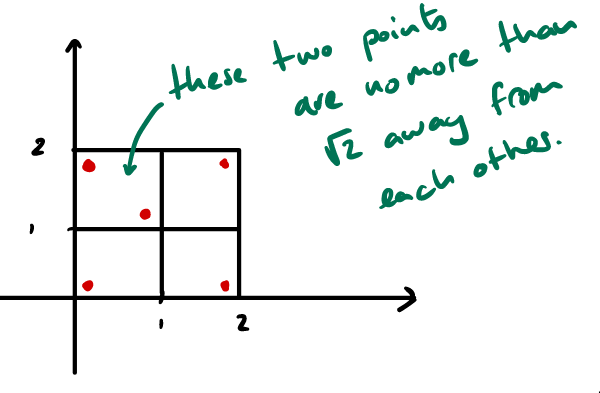
\includegraphics[scale=0.5]{ex.png}
    \end{center}

    \pagebreak
    \section{(5.6) Function Composition and Inverse Functions}

    \subsection{Bijective functions}

    If \(f: A \rightarrow B\), then $f$ is said to be \emph{bijective}, or to be a \emph{one-to-one corespondence}, if $f$ is both one-to-one and onto.

    \subsection{Identity function}

    The function \(1_A : A \rightarrow A\), defined by \(1_A (a) = a\) for all \(a \in A\), is called the \emph{identity function}.

    \subsection{Equality of functions}

    If \(f,g : A \rightarrow B\), we say that $f$ and $g$ are \emph{equal} and write \(f = g\), if \(f(a) = g(a)\) for all \(a \in A\).

    A common pitfall in dealing with the equality of functions occurs when $f$ and $g$ are functions with a common domain $A$ and \(f(a) = g(a)\) for all \(a \in A\). It may \emph{not} be the case that \(f = g\). The pitfall results from not paying attention to the codomains of the functions.

    \subsubsection{Example}

    Let \(f: \mathbb{Z} \rightarrow \mathbb{Z}, g: \mathbb{Z} \rightarrow \mathbb{Q}\) where \(f(x) = x = g(x)\), for all \(x \in \mathbb{Z}\). Then, \(f,g \) share the common domain \(\mathbb{Z}\), have the same range \(\mathbb{Z}\), and act the same on every element of \(\mathbb{Z}\). Yet \(f \neq g\) because $f$ is injective and $g$ is injective but surjective; so the codomains do not make a difference.

    \subsection{Composite functions}

    If \(f:A \rightarrow B\) and \(g: B \rightarrow C\), we define the \emph{composite function}, which is denoted \(g \circ f: A \rightarrow C\), by \((g \circ f)(a) = g(f(a))\), for each \(a \in A\). $f$ and $g$ are composable. However, if \(C \neq A\) then \(f \circ g\) is not defined.

    \vspace{1em}

    The definition and examples for composite functions required that the codomain of $f$ = domain of $g$. If range of $f$ \(\subseteq\) $g$, this will actually be enough to yield the composite function \(g \circ f: A \rightarrow C\). Also, for any \(f:A \rightarrow B\), we observe that \(f \circ 1_A = f = 1_B \circ f\).

    \subsubsection{Theorem}

    Let \(f:A \rightarrow B\) and \(g:B \rightarrow C\).
    \begin{enumerate}
        \item[(a)] If  $f$ and $g$ are one-to-one, then \(g \circ f\) is one-to-one.
        \item[(b)] If $f$ and $g$ are onto, then \(g \circ f\) is onto.   
    \end{enumerate}

    \begin{proof} Let us prove the following theorem above.
        \begin{enumerate}
            \item[(a)] Let \(a_1, a_2 \in A\) with \((g \circ f)(a_1) = (g \circ f)(a_2)\). Then \[(g \circ f)(a_1) = (g \circ f)(a_2) \Rightarrow g(f(a_1)) = g(f(a_2)) \Rightarrow f(a_1) = f(a_2)\] since $g$ is one-to-one. Also, \(a_1 = a_2\) because $f$ is one-to-one. Consequently, \(g \circ f\) is one-to-one. 
            \item[(b)] Let \(z \in C\). Since $g$ is onto, there exists \(y \in B\) with \(g(y) = z.\) With $f$ onto and \(y \in B\), there exists \(x \in A\) with \(f(x) = y\). Hence, \(z = g(y) = g(f(x)) = (g \circ f)(x)\), so the range of \(g \circ f = C = \) the codomain of \(g \circ f\), and \(g \circ f\) is onto. 
        \end{enumerate}
    \end{proof}

    Function composition is not commutative, but it is associative.

    \subsubsection{Collection of functions}

    If $A$ is a set then \[A^A = \{f \mid f:A \rightarrow A\}\] is the collection of functions \(A \rightarrow A\). So the function composition is a binary operation on $A^A$.

    \subsubsection{Theorem}

    If \(f: A \rightarrow B, g: B \rightarrow C\), and \(h:C \rightarrow D\), then \[ (h \circ g) \circ f = h \circ (g \circ f). \]

    \begin{proof}
        We have \[(h \circ g) \circ f(x) = h(g(f(x)))\] and \[h \circ (g \circ f)(x) = h(g(f(x))).\] Therefore, we have \((h \circ g) \circ f = h \circ (g \circ f).\)
    \end{proof}

    \subsubsection{Powers of functions}

    If \(f:A \rightarrow A\), we define \(f^1 = 1\), and for \(n \in \mathbb{Z}^+, f^{n+1} = f \circ f(^n).\)

    \vspace{1em}

    This definition is another example wherein the result is defined \emph{recursively}. With \(f^{n+1} = f \circ (f^n)\), we see the dependence of \(f^{n+1}\) on a previous power, namely, \(f^n\).

    \subsection{Invertible functions}

    \subsubsection{Converse of a relation}

    For sets \(A,B,\) if $R$ is a relation from $A$ to $B$, then the \emph{converse} of $R$, denoted $R^c$, is the relation from $B$ to $A$ defined by \[R^c = \{(b,a) \mid (a,b) \in R\}.\] We simply interchange the components of each ordered pair in $R$.

    \subsubsection{Invertible function}

    If \(f:A \rightarrow B\), then $f$ is said to be \emph{invertible} if there is a function \(g: B \rightarrow A\) such that \(g \circ f = 1_A\) and \(f \circ g = 1_B.\)

    \subsubsection{Uniqueness}

    If a function \(f: A \rightarrow B\) is invertible and a function \(g:B \rightarrow A\) satisfies \(g \circ f = 1_A\) and \(f \circ g = 1_B\), then this function $g$ is unique.

    \begin{proof}
        If $g$ is not unique, then there is another function \(h: B \rightarrow A\) with \(h \circ f = 1_A\) and \(f \circ h = 1_B \). Consequently, \[h = h \circ 1_B = h \circ (f \circ g) = (h \circ f) \circ g = 1_A \circ g = g.\]
    \end{proof}

    As a result of this theorem, we shall call the function $g$ the inverse of $f$ and shall adopt the notation \(g = f^{-1}\). Note that \(f^{-1} = f^c\) and \((f^{-1})^{-1} = f.\)

    \subsubsection{Theorem}

    \(f: A \rightarrow B\) is invertible if and only if $f$ is bijective. 
    \begin{proof}
        Assuming that $f$ is invertible, we have a unique function \(g:B \rightarrow A\) with \(g \circ f = 1_A, f \circ g = 1_B\). If \(a_1,a_2 \in A\) with \(f(a_1) = f(a_2)\), then \(g(f(a_1)) = g(f(a_2))\). It follows that \(a_1 = a_2\), so $f$ is one-to-one. For the onto property, let \(b \in B\), then \(g(b) \in A\). We have \(b = 1_B (b) = (f \circ g)(b) = f(g(b))\), so $f$ is onto.

        \vspace{1em}

        For the other direction, suppose \(f: A \rightarrow B\) is bijective. Since $f$ is onto, for each \(b \in B\), there is an  \(a \in A\) with \(f(a) = b.\) Consequently, we define the function \(g: B \rightarrow A\) by \(g(b) = a\), where \(f(a) = b\). Our definition of $g$ such that \(g \circ f = 1_A\) and \(f \circ g = 1_B\), so we find that $f$ is invertible, with \(g = f^{-1}\).
    \end{proof}

    \subsubsection{Theorem}

    If \(f:A \rightarrow B, g:B \rightarrow C\) are invertible functions, then \(g \circ f: A \rightarrow C\) is invertible and \[(g \circ f)^{-1} = f^{-1} \circ g^{-1}.\]

    \subsection{Inverse image}

    If \(f: A \rightarrow B\) and \(B_1 \subseteq B\), then \(f^{-1} (B_1) = \{x \in A \mid f(x) \in B_1\}\). The set \(f^{-1}(B_1)\) is called the \emph{preimage or inverse image} of $B_1$ under $f$.

    \vspace{1em}

    \emph{Note.} \(f^{-1}(B_1)\) is defined even if $f$ is not invertible. 

    \subsubsection{Examples}

    \begin{itemize}
        \item For \(f: \mathbb{Z} \rightarrow \mathbb{Z}\), we have \[f^{-1}[\{2\}] = \{2\}.\]
        \item For \(f: \mathbb{Z} \rightarrow \mathbb{Z}\), we have \[f^{-1}[\{0\}] = \{x \in \mathbb{Z} \mid f(x) \in \{0\}\} = \{x \in \mathbb{Z} \mid f(x) = 0\}\] and \[f^{-1}[\{1,2\}] = \emptyset.\]
        \item For \(f: \mathbb{Z} \rightarrow \mathbb{Z}_2\), we have \[f^{-1}[\{0\}] = 2 \mathbb{Z} \qquad \text{even integers}\] and \[f^{-1}[\{1\}] = 2 \mathbb{Z} + 1 \qquad \text{odd integers}\]
    \end{itemize}

    \subsection{Theorem}

    If \(f: A \rightarrow B\) and \(B_1, B_2 \subseteq B\), then 
    \begin{enumerate}
        \item[(a)] \(f^{-1}(B_1 \cap B_2) = f^{-1}(B_1) \cap f^{-1}(B_2)\);
        \item[(b)] \(f^{-1}(B_1 \cup B_2) = f^{-1}(B_1) \cup f^{-1}(B_2);\)
        \item[(c)] \(f^{-1}(\overline{B_1}) = \overline{f^{-1}(B_1)}\).   
    \end{enumerate}

    \subsection{Finite sets}

    Let \(f: A \rightarrow B\) for finite sets $A$ and $B$, where \(|A| = |B|\). Then the following statements are equivalence: (a) $f$ is one-to-one; (b) $f$ is onto; and (c) $f$ is invertible.
    
\end{document}